\documentclass[a4paper]{article}
\usepackage{graphicx}
% Set target color model to RGB
\usepackage[inner=1.5cm,outer=1.5cm,top=1.5cm,bottom=2.5cm]{geometry}
\usepackage{setspace}
\usepackage[rgb]{xcolor}
\usepackage{amsgen,amsmath,amstext,amsbsy,amsopn,amssymb}
\usepackage[colorlinks=true, urlcolor=blue,  linkcolor=blue, citecolor=blue]{hyperref}
\usepackage{enumitem}
\usepackage{dsfont}
\usepackage{multirow}
\usepackage{float} % in the preamble
\usepackage{booktabs}
\newcommand{\ra}[1]{\renewcommand{\arraystretch}{#1}}

\newcommand{\project}[4]{
   \pagestyle{myheadings}
   \thispagestyle{plain}
   \newpage
   \setcounter{page}{1}
   \noindent
   \begin{center}
   \framebox{
      \vbox{\vspace{2mm}
    % \hbox to 6.28in { {\bf MLR \hfill} }
       \vspace{6mm}
       \hbox to 6.28in { {\Large \hfill {#1} #2  \hfill} }
       \vspace{6mm}
       \hbox to 6.28in { {\it Student: #3 \hfill } }
    %    \hbox to 6.28in { {\it Student 2: #4 \hfill }}
      \vspace{2mm}}
   }
   \end{center}
   \vspace*{4mm}
}
\title{Push \& Learn}

% Path to images
\graphicspath{{../src/results/}}

\begin{document}
\project{Project 2}{: Push \& Learn --- Learning Dynamics Through Learning}{Shibani, Senthilbabu}{}


%=============================================================================
\section{Introduction}
%=============================================================================

This report presents the implementation and evaluation of three models for predicting the planar motion of a cracker box pushed by a robotic manipulator. Given push parameters $(\theta_0, d, D)$---the initial orientation, contact offset, and push distance---the goal is to predict the resulting change in position and orientation $(\Delta x, \Delta y, \Delta\theta)$ of the object. We compare:

\begin{enumerate}
    \item A \textbf{physics-based model} derived from rigid-body dynamics,
    \item A \textbf{neural network model} (MLP) trained purely from data,
    \item A \textbf{hybrid model} that augments physics predictions with a learned correction network.
\end{enumerate}

Data is generated from the Genesis simulator for a cracker box object. The dataset consists of input features $\mathbf{x} = [\theta_0, d, D]$ and ground-truth outputs $\mathbf{y} = [\Delta x, \Delta y, \Delta\theta]$ in the global frame. An 80/20 train/validation split with a fixed random seed of 42 is used throughout.


%=============================================================================
\section{Physics-Based Model (30 points)}
%=============================================================================

\subsection{Formulation}

The physics model implements the equations provided in the project appendix and clarification document. Given push parameters $(\theta_0, d, D)$ and a push duration $T = 3$~s, we perform numerical integration over $N = 300$ timesteps ($\Delta t = 0.01$~s).

\subsubsection{Velocity Profile}

A sinusoidal profile ensures smooth acceleration and deceleration:
\begin{equation}
    v(t) = \frac{v_{\max}}{2}\left(\sin\!\left(\frac{2\pi t}{T} - \frac{\pi}{2}\right) + 1\right), \qquad v_{\max} = \frac{2D}{T}.
\end{equation}

\subsubsection{Angular Motion}

We implement the rotational dynamics from first principles using Newton's second law for rotation. The pushing force $F = m \cdot v(t)$ applied at offset $d$ from the center of mass produces a torque:
\begin{equation}
    \tau_i = m \cdot v_i \cdot d \qquad [\text{N}{\cdot}\text{m}].
\end{equation}
The angular acceleration follows from $\tau = I\alpha$, where $I = \tfrac{1}{12}ms^2$ is the moment of inertia for a square object of mass $m$ and side length $s$:
\begin{equation}
    \alpha_i = \frac{\tau_i}{I} = \frac{m \cdot v_i \cdot d}{\tfrac{1}{12}ms^2} = \frac{12 \, v_i \, d}{s^2} \qquad [\text{rad/s}^2].
\end{equation}
The angular position is updated using the kinematic equation:
\begin{equation}
    \Delta\theta_i = \tfrac{1}{2}\,\alpha_i \, \Delta t^2 \qquad [\text{rad}], \qquad \theta_i = \theta_{i-1} + \Delta\theta_i.
\end{equation}
Every term is dimensionally consistent: $\tau$ in N$\cdot$m, $\alpha$ in rad/s$^2$, and $\Delta\theta$ in radians. No fitted scaling parameters are used---the physics constants ($m = 0.1$~kg, $s = 0.1$~m) are taken directly from the configuration.

\subsubsection{Linear Motion and Frame Transformation}

Position updates follow the appendix equations in the local frame:
\begin{equation}
    \Delta x_i = -v_i \cos(\theta_i) \cdot \Delta t, \qquad \Delta y_i = -v_i \sin(\theta_i) \cdot \Delta t.
\end{equation}

Local-frame displacements are then transformed to the global frame via the rotation matrix:
\begin{equation}
    \begin{bmatrix} x_{\text{global}} \\ y_{\text{global}} \end{bmatrix}
    = \begin{bmatrix} \cos\theta_0 & -\sin\theta_0 \\ \sin\theta_0 & \cos\theta_0 \end{bmatrix}
    \begin{bmatrix} x_{\text{local}} \\ y_{\text{local}} \end{bmatrix}.
\end{equation}

The final predicted state is $\mathbf{s}_{\text{predicted}} = [x_{\text{global}},\; y_{\text{global}},\; \theta_{\text{final}}]$.

\subsection{Results}

The physics model achieves a validation MSE of \textbf{0.171645}. The per-dimension breakdown (Figure~\ref{fig:per_dim}) reveals that nearly all error comes from the angular dimension ($d\theta$ MSE $= 0.505705$), while positional errors are comparatively small ($dx$ MSE $= 0.006011$, $dy$ MSE $= 0.003219$). The model severely under-predicts rotation: over 10 sequential pushes (Figure~\ref{fig:physics_traj}), the predicted cumulative orientation barely reaches $-30°$ while the ground truth reaches $-230°$.

This large angular error is expected. The idealized model assumes a point contact, rigid-body inertia $I = \tfrac{1}{12}ms^2$ for a square object, and no friction losses. In reality, the cracker box is rectangular (not square), contact is distributed across a face, and surface friction dissipates energy and alters the effective torque. These unmodeled effects explain the order-of-magnitude discrepancy in angular prediction, and motivate the use of data-driven models to correct or replace the physics.

\begin{figure}[H]
    \centering
    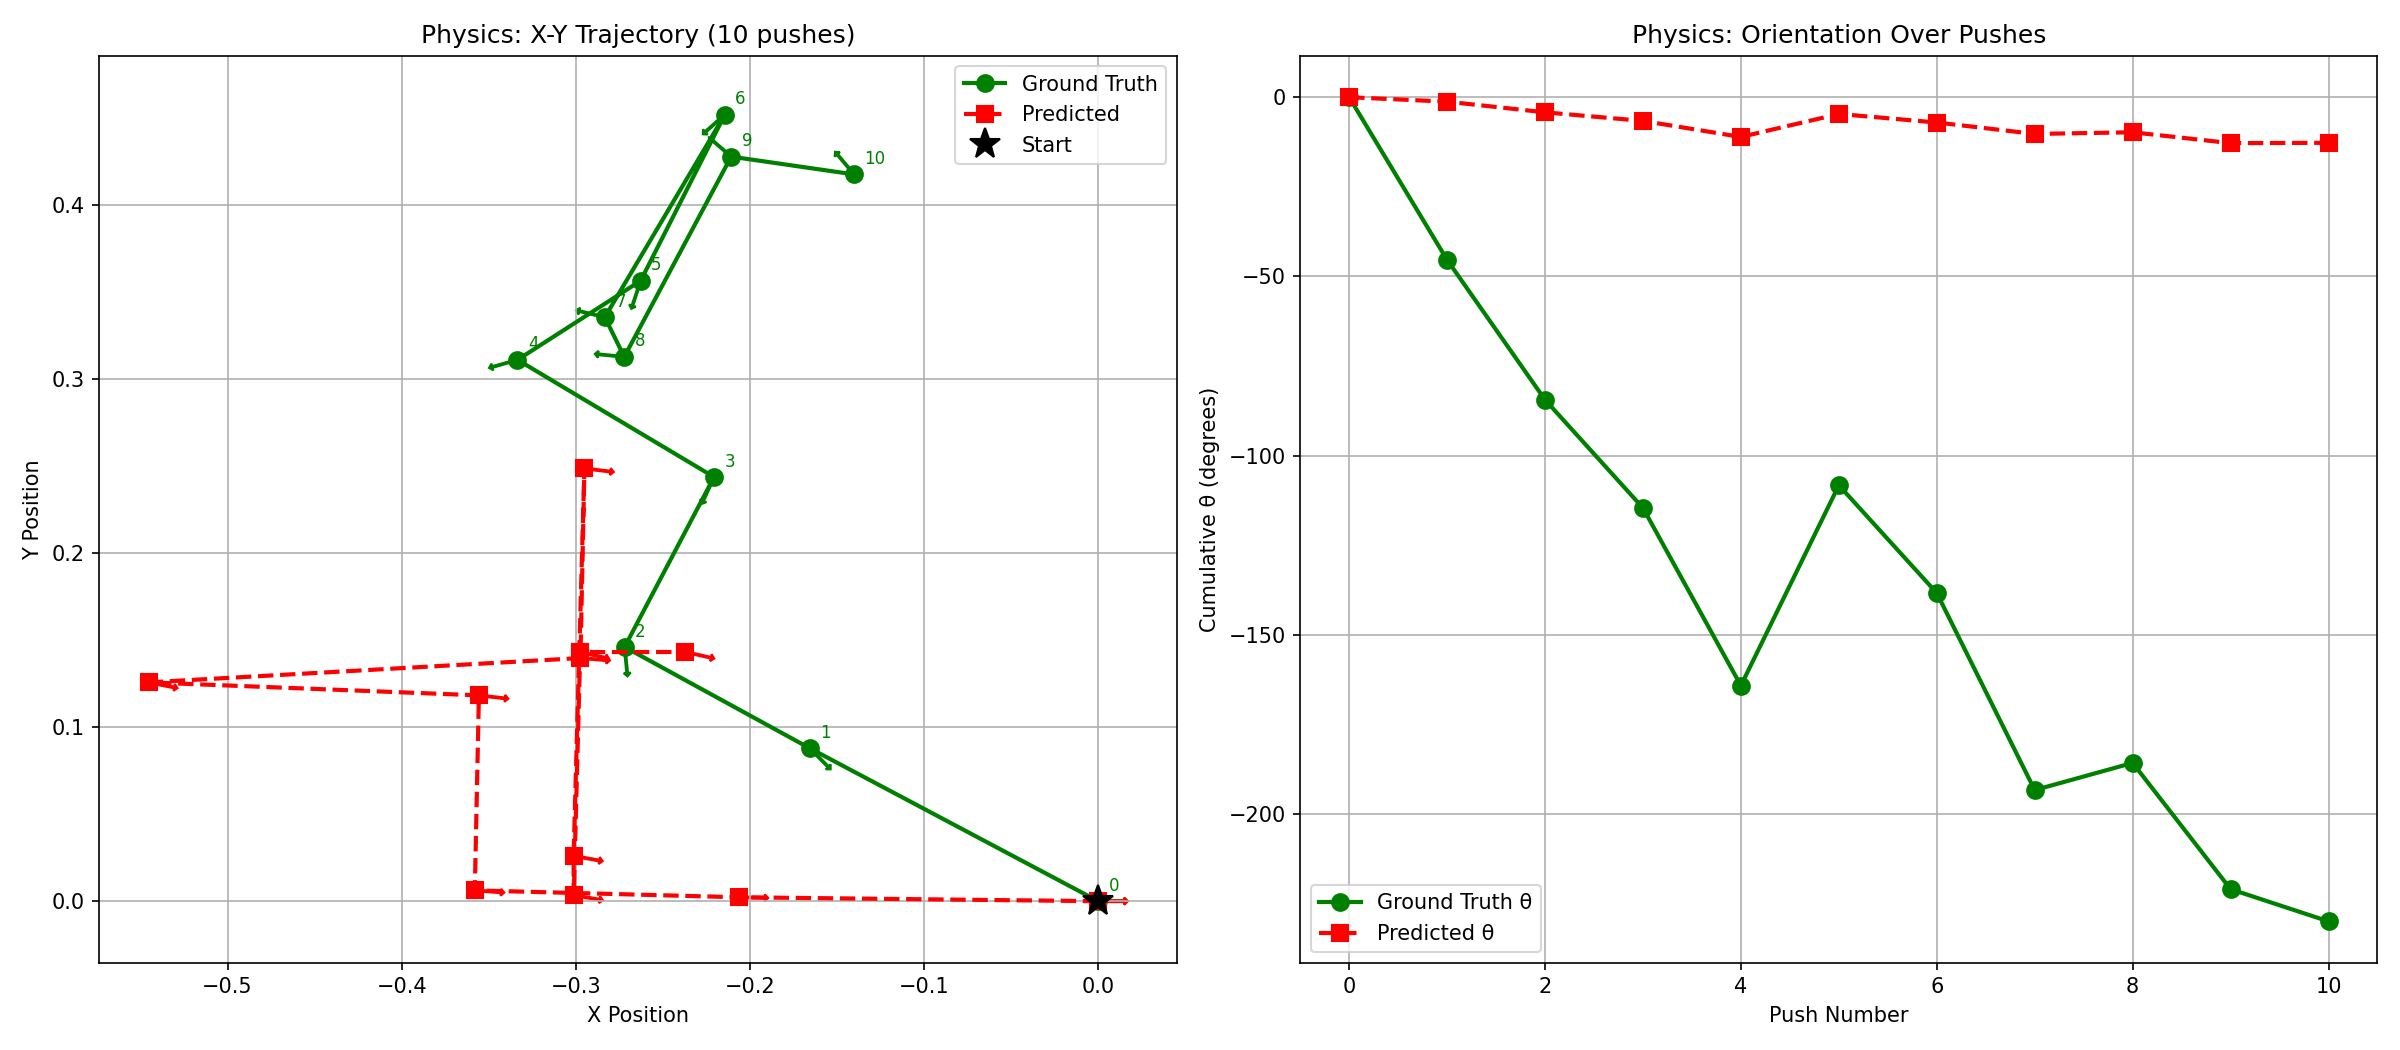
\includegraphics[width=0.85\textwidth]{physics_trajectory.png}
    \caption{Physics model trajectory over 10 sequential pushes. Left: X-Y path with orientation arrows. Right: Cumulative orientation. The predicted trajectory (red) diverges significantly from ground truth (green), particularly in orientation.}
    \label{fig:physics_traj}
\end{figure}


%=============================================================================
\section{Neural Network Model (30 points)}
%=============================================================================

\subsection{Feature Engineering}

Raw 3D inputs $[\theta_0, d, D]$ are expanded into a 20-dimensional feature vector to capture nonlinear, periodic relationships:

\begin{itemize}
    \item Raw inputs (3 features)
    \item Trigonometric harmonics: $\sin(k\theta_0), \cos(k\theta_0)$ for $k = 1, 2, 3, 4$ (8 features)
    \item Quadratic terms: $d^2, D^2$ (2 features)
    \item Cross-product: $d \cdot D$ (1 feature)
    \item Interaction terms: $d \cdot \sin\theta_0$, $d \cdot \cos\theta_0$, $D \cdot \sin\theta_0$, $D \cdot \cos\theta_0$ (4 features)
    \item Triple interactions: $d \cdot D \cdot \sin\theta_0$, $d \cdot D \cdot \cos\theta_0$ (2 features)
\end{itemize}

The higher-order harmonics (up to $4\theta_0$) are motivated by the periodic dependence of push dynamics on the object's orientation.

\subsection{Architecture}

The network is a two-hidden-layer MLP with input/output normalization:
\[
    20 \xrightarrow{\text{Linear}} 64 \xrightarrow{\text{ReLU}} 64 \xrightarrow{\text{ReLU}} 3
\]
Input features are normalized to zero mean and unit variance using training-set statistics. Outputs are denormalized as $\hat{y} = \hat{y}_{\text{norm}} \cdot \sigma_y + \mu_y$ to produce predictions in the original scale.

\subsection{Training Procedure}

\begin{itemize}
    \item \textbf{Optimizer}: Adam with learning rate $\eta = 0.001$ and weight decay $\lambda = 10^{-4}$
    \item \textbf{Scheduler}: Linear warmup over 50 epochs, then cosine annealing
    \item \textbf{Loss}: Mean Squared Error: $\mathcal{L} = \frac{1}{N}\sum_{i=1}^{N} \|\mathbf{s}_{\text{pred}}^{(i)} - \mathbf{s}_{\text{final}}^{(i)}\|^2$
    \item \textbf{Gradient clipping}: Max norm of 1.0
    \item \textbf{Early stopping}: Patience of 500 epochs on validation loss
    \item \textbf{Batch size}: 64 with shuffling
    \item \textbf{Maximum epochs}: 3000
\end{itemize}

After Adam training converges, we apply \textbf{L-BFGS fine-tuning}---a full-batch, second-order optimizer with Strong Wolfe line search (learning rate 0.1, up to 1000 iterations). This refines the model to a better local optimum by exploiting curvature information.

\subsection{Results}

The NN model achieves a validation MSE of approximately \textbf{0.000296}---a \textbf{580$\times$ improvement} over the physics model. Per-dimension errors are dramatically reduced: $dx$ MSE $= 2.4 \times 10^{-5}$, $dy$ MSE $= 1.3 \times 10^{-5}$, $d\theta$ MSE $= 8.51 \times 10^{-4}$ (Figure~\ref{fig:per_dim}). Training converges rapidly within $\sim$200 epochs (Figure~\ref{fig:training_curves}), and the overfitting gap is negligible (Figure~\ref{fig:overfitting}), indicating strong generalization.

\begin{figure}[H]
    \centering
    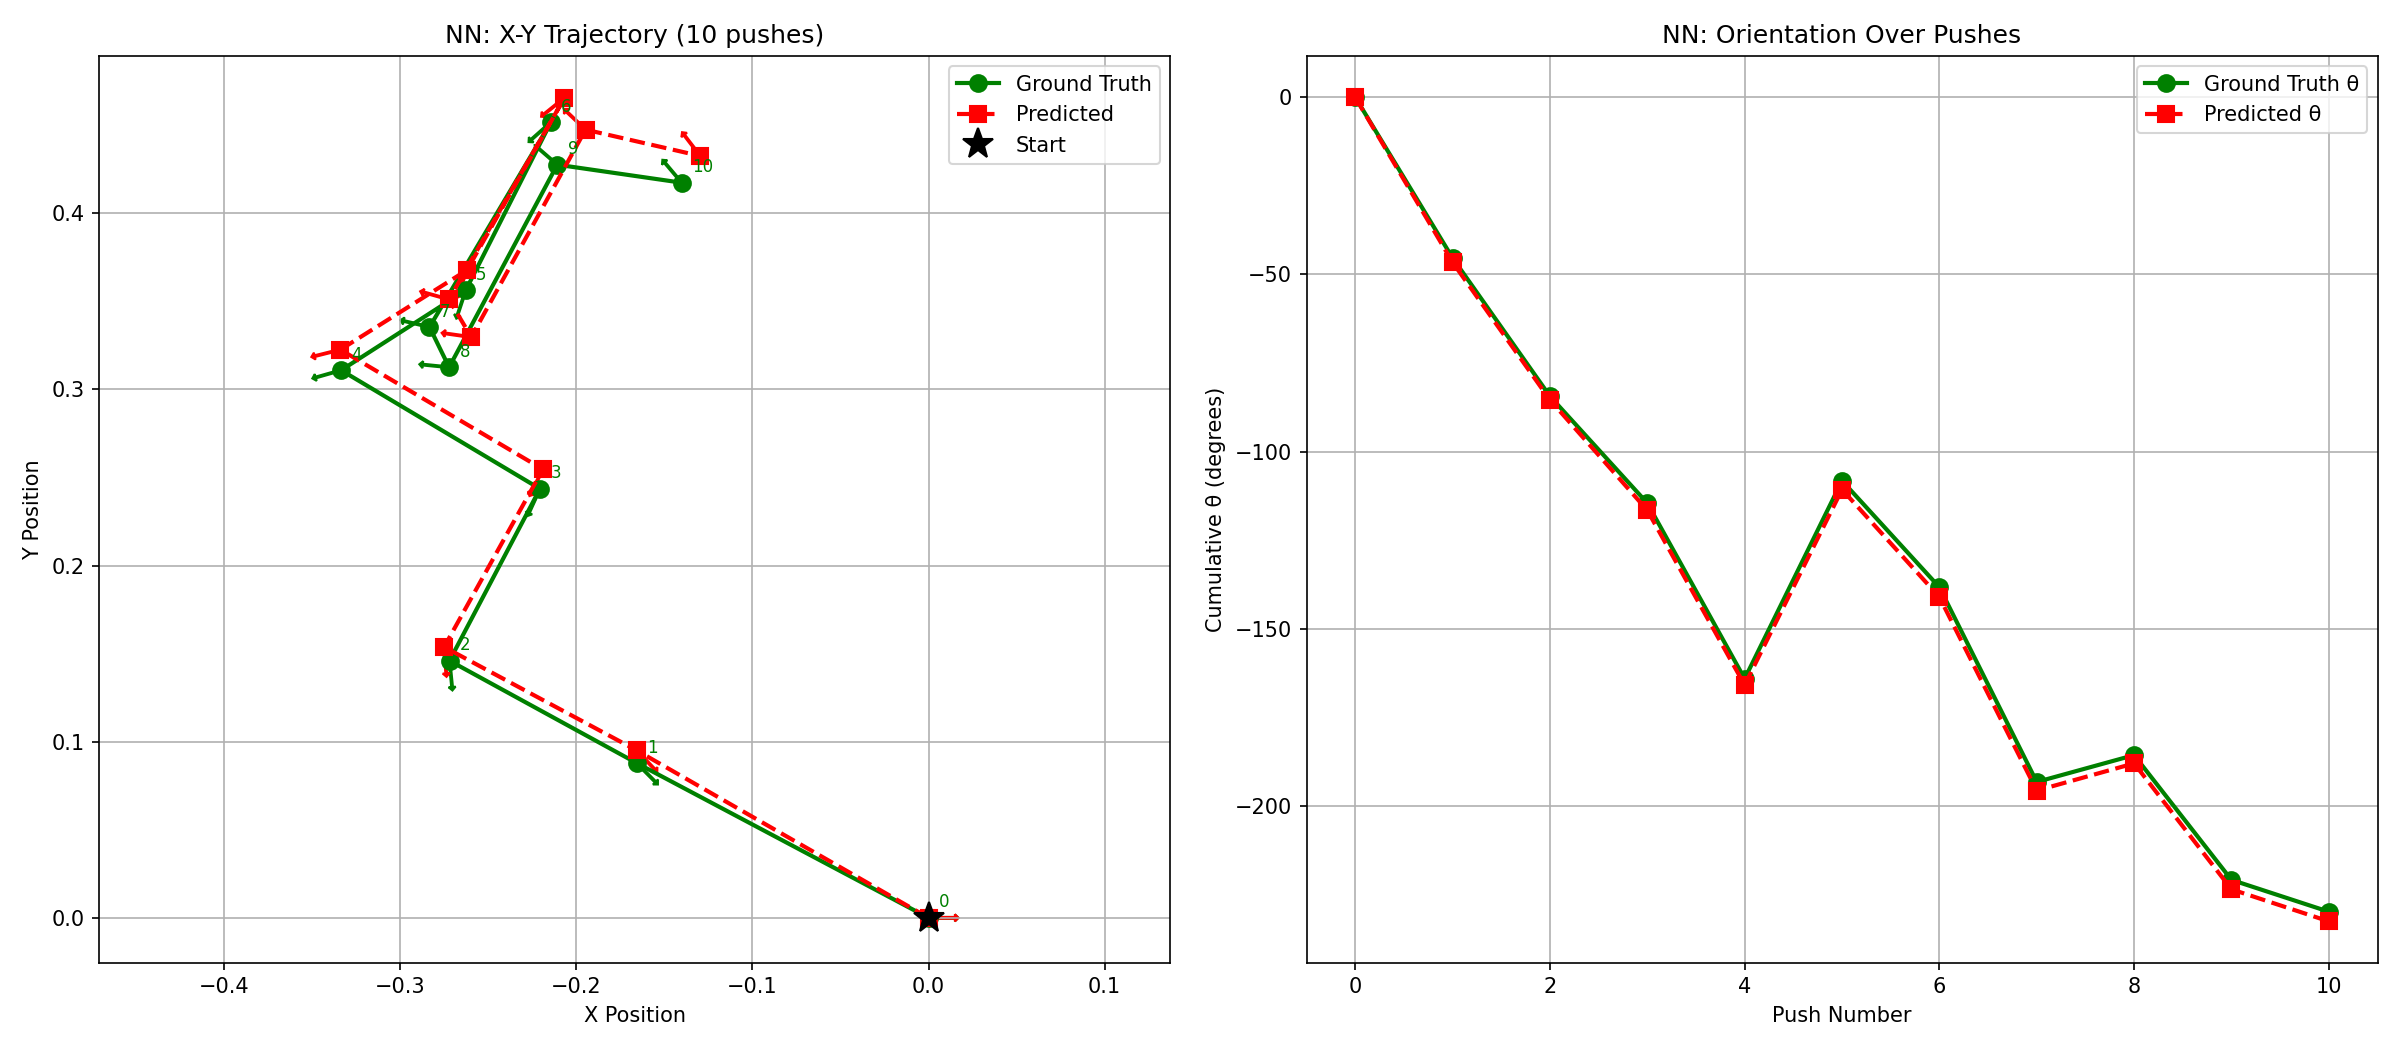
\includegraphics[width=0.85\textwidth]{nn_trajectory.png}
    \caption{NN model trajectory over 10 sequential pushes. The predicted path (red) closely follows the ground truth (green) in both position and orientation, with only minor accumulated errors at later pushes.}
    \label{fig:nn_traj}
\end{figure}


%=============================================================================
\section{Hybrid Physics + Neural Network Model (40 points)}
%=============================================================================

\subsection{Architecture}

The hybrid model uses the physics model's predictions as additional input features to the neural network. The key insight is that the network learns a \textit{residual correction} to the physics prediction, rather than learning the full mapping from scratch.

\subsubsection{Input Augmentation}

The raw push parameters are first passed through the physics engine to obtain $\hat{\mathbf{y}}_{\text{phys}} = [\Delta\hat{x}, \Delta\hat{y}, \Delta\hat{\theta}]_{\text{phys}}$. These 3 physics predictions are normalized and concatenated with the 20 engineered features to form a 23-dimensional input. Physics predictions are cached during training for computational efficiency.

\subsubsection{Correction Network}

\[
    [\text{feat}_{\text{norm}}(20);\; \text{phys}_{\text{norm}}(3)] \xrightarrow{\text{Linear}} 64 \xrightarrow{\text{ReLU}} 64 \xrightarrow{\text{ReLU}} 3
\]

The final output uses a residual formulation:
\begin{equation}
    \hat{\mathbf{y}} = \hat{\mathbf{y}}_{\text{phys}} + \mathbf{c}_{\text{norm}} \cdot \sigma_y,
\end{equation}
where $\mathbf{c}_{\text{norm}}$ is the network's normalized correction output and $\sigma_y$ is the per-dimension output standard deviation. This design ensures the network only needs to model the \textit{error} of the physics model, which has lower variance than the raw dynamics, simplifying the learning problem.

\subsection{Training}

The hybrid model uses the same training procedure as the NN model: Adam optimizer with warmup-cosine schedule, early stopping with patience 500, gradient clipping at 1.0, followed by L-BFGS fine-tuning with identical hyperparameters.

\subsection{Results}

The hybrid model achieves a validation MSE of approximately \textbf{0.000262}---a \textbf{655$\times$ improvement} over the physics model and a \textbf{1.1$\times$ improvement} over the pure NN. The most notable gain is in the angular dimension: $d\theta$ MSE drops from $8.51 \times 10^{-4}$ (NN) to $6.09 \times 10^{-4}$ (Hybrid), a 28\% reduction (Figure~\ref{fig:per_dim}). Even though the physics model itself is inaccurate, its predictions still provide structural information (e.g., the sign and rough scale of motion) that helps the correction network converge to a better solution.

\begin{figure}[H]
    \centering
    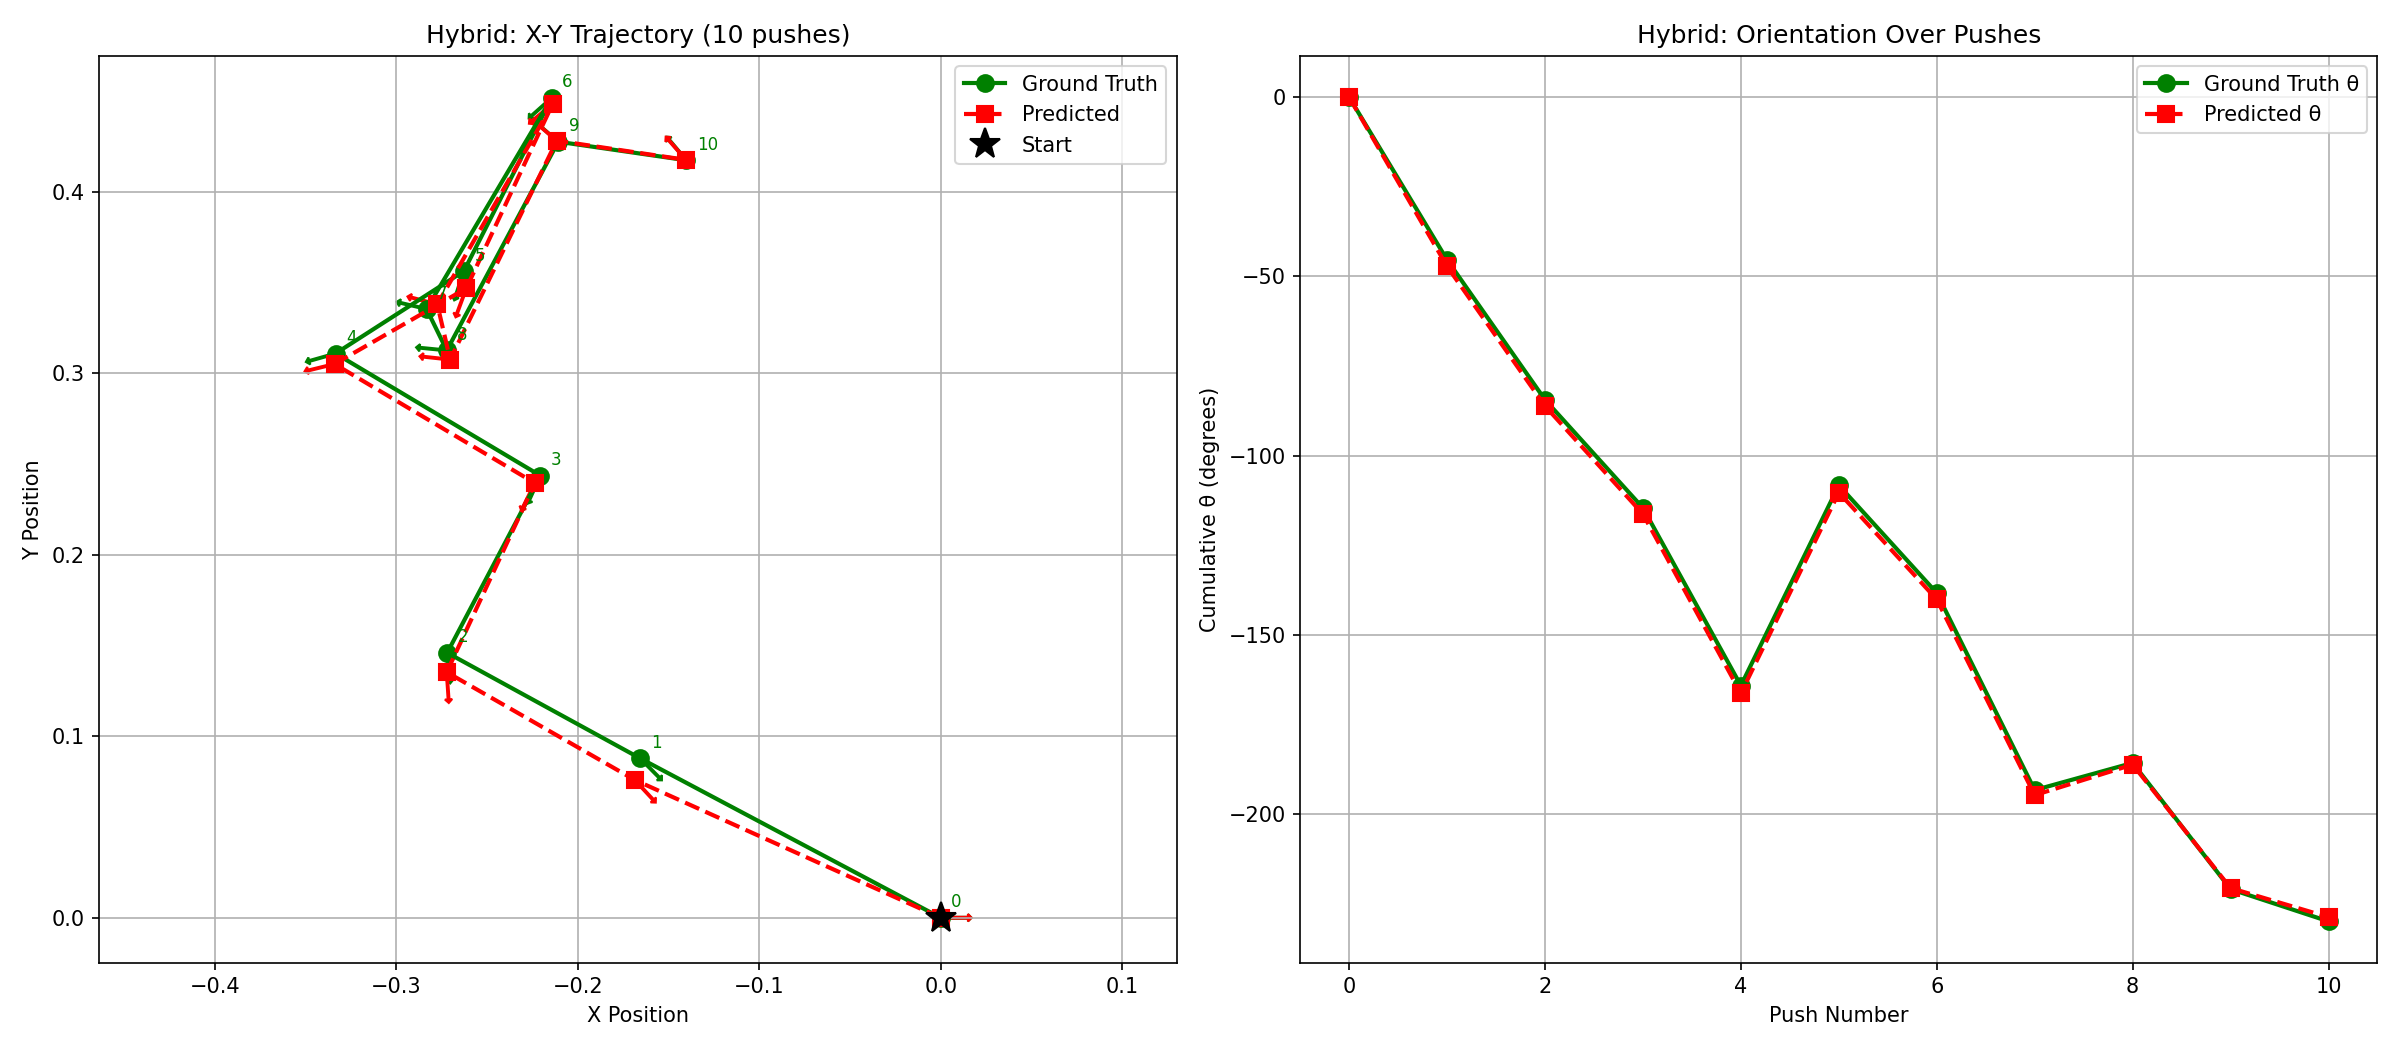
\includegraphics[width=0.85\textwidth]{hybrid_trajectory.png}
    \caption{Hybrid model trajectory over 10 sequential pushes. The closest match to ground truth among all three models, with excellent orientation tracking throughout the full sequence.}
    \label{fig:hybrid_traj}
\end{figure}


%=============================================================================
\section{Evaluation and Discussion}
%=============================================================================

\subsection{Quantitative Comparison}

Table~\ref{tab:results} summarizes the validation MSE for all three models.

\begin{table}[H]
\centering
\ra{1.3}
\caption{Validation MSE comparison across all three models.}
\label{tab:results}
\begin{tabular}{@{}lccccc@{}}
\toprule
\textbf{Model} & \textbf{Total MSE} & $\boldsymbol{dx}$ \textbf{MSE} & $\boldsymbol{dy}$ \textbf{MSE} & $\boldsymbol{d\theta}$ \textbf{MSE} & \textbf{Improvement} \\
\midrule
Physics          & 0.171645 & 0.006011 & 0.003219 & 0.505705 & --- \\
Neural Network   & 0.000296 & 0.000024 & 0.000013 & 0.000851 & $580\times$ \\
Hybrid (NN+Phys) & 0.000262 & 0.000132 & 0.000045 & 0.000609 & $655\times$ \\
\bottomrule
\end{tabular}
\end{table}

\subsection{Training Curves and Generalization}

\begin{figure}[H]
    \centering
    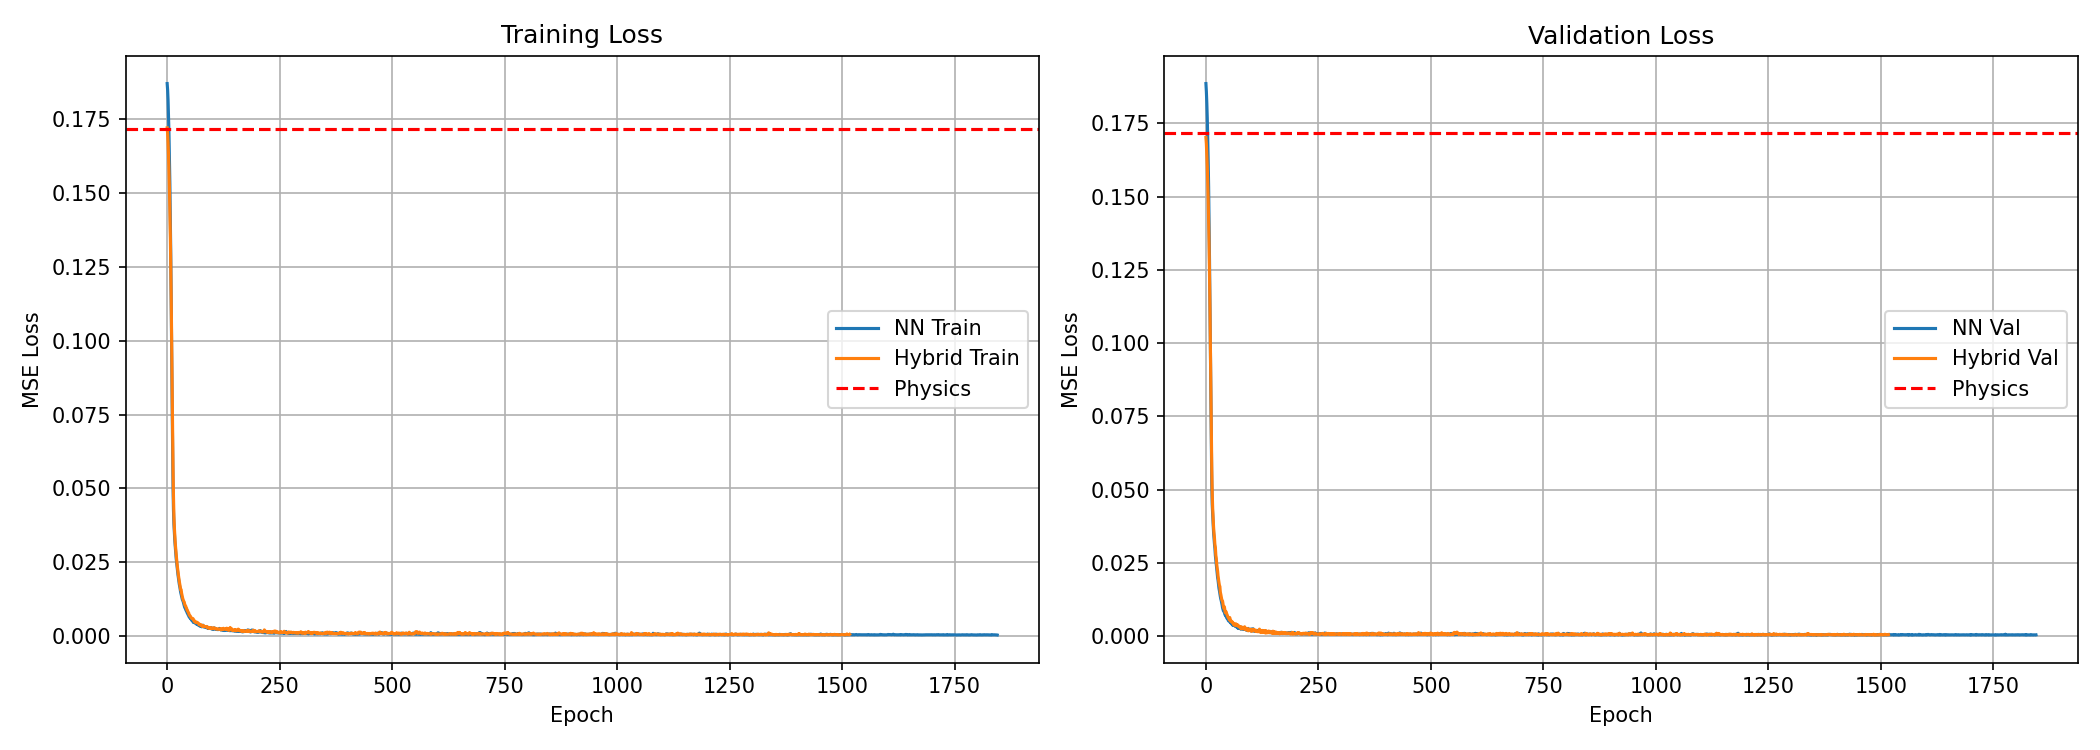
\includegraphics[width=\textwidth]{training_curves.png}
    \caption{Training and validation loss curves for the NN and Hybrid models. The red dashed line indicates the physics model's validation MSE. Both learned models converge well below the physics baseline. The NN starts from a higher initial loss but converges quickly; the Hybrid model starts closer to the physics MSE and converges smoothly.}
    \label{fig:training_curves}
\end{figure}

\begin{figure}[H]
    \centering
    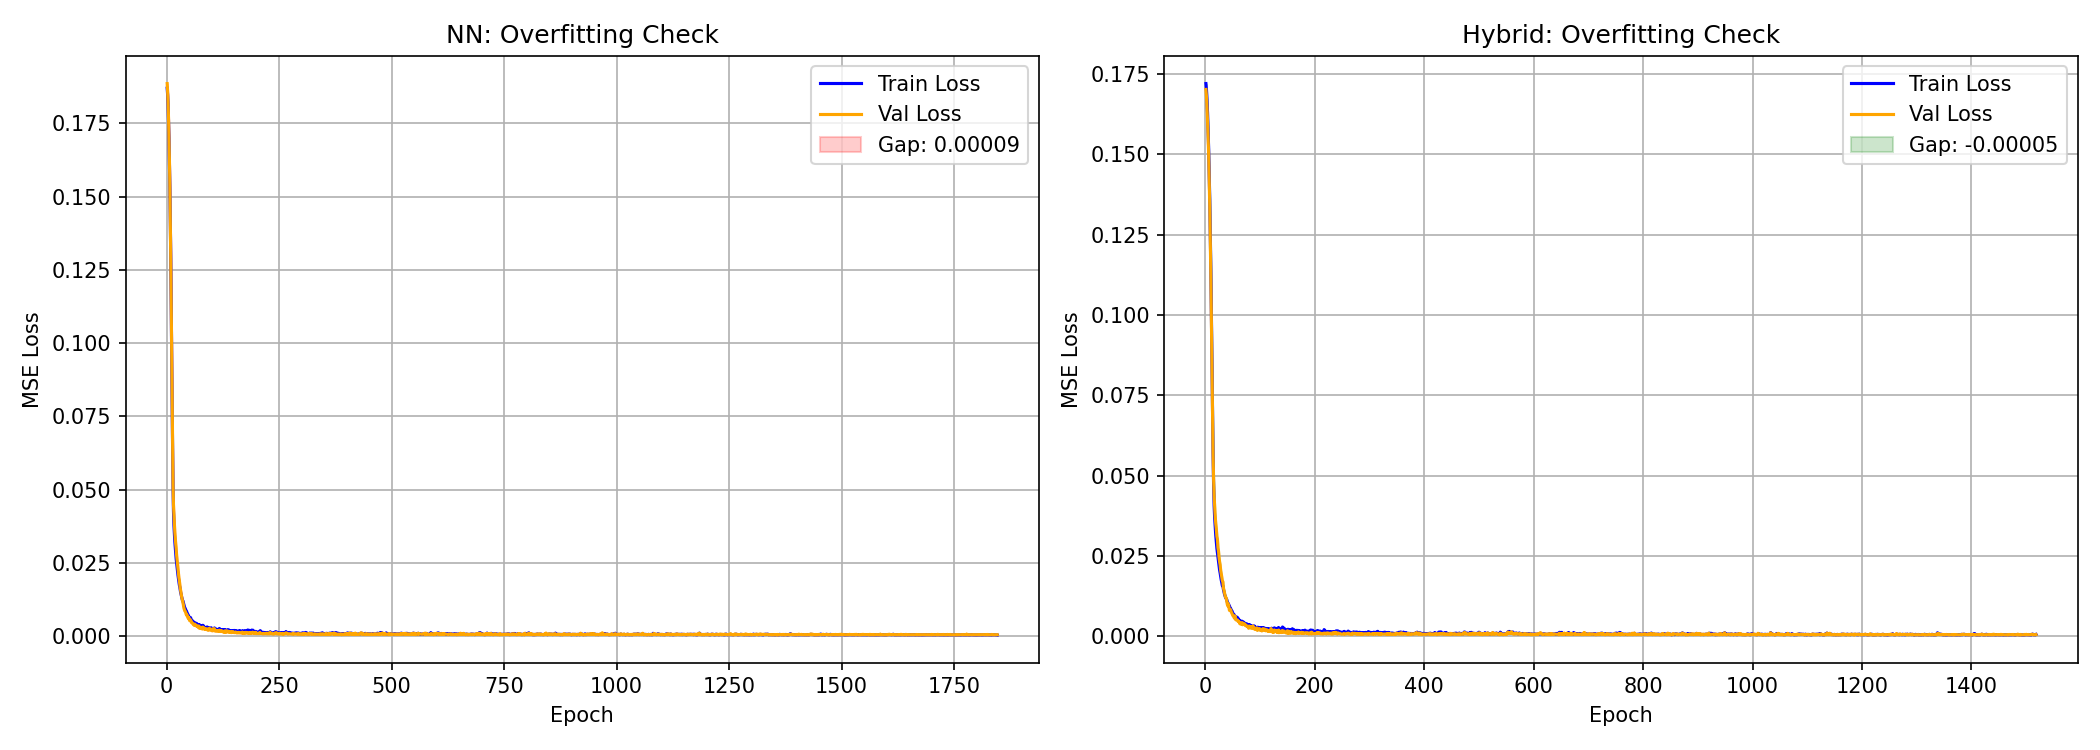
\includegraphics[width=\textwidth]{overfitting_check.png}
    \caption{Overfitting analysis. The NN model (left) has a train-val gap of $9 \times 10^{-5}$ and the Hybrid model (right) has a gap of $1 \times 10^{-4}$. Both gaps are negligible, confirming good generalization without overfitting.}
    \label{fig:overfitting}
\end{figure}

\begin{figure}[H]
    \centering
    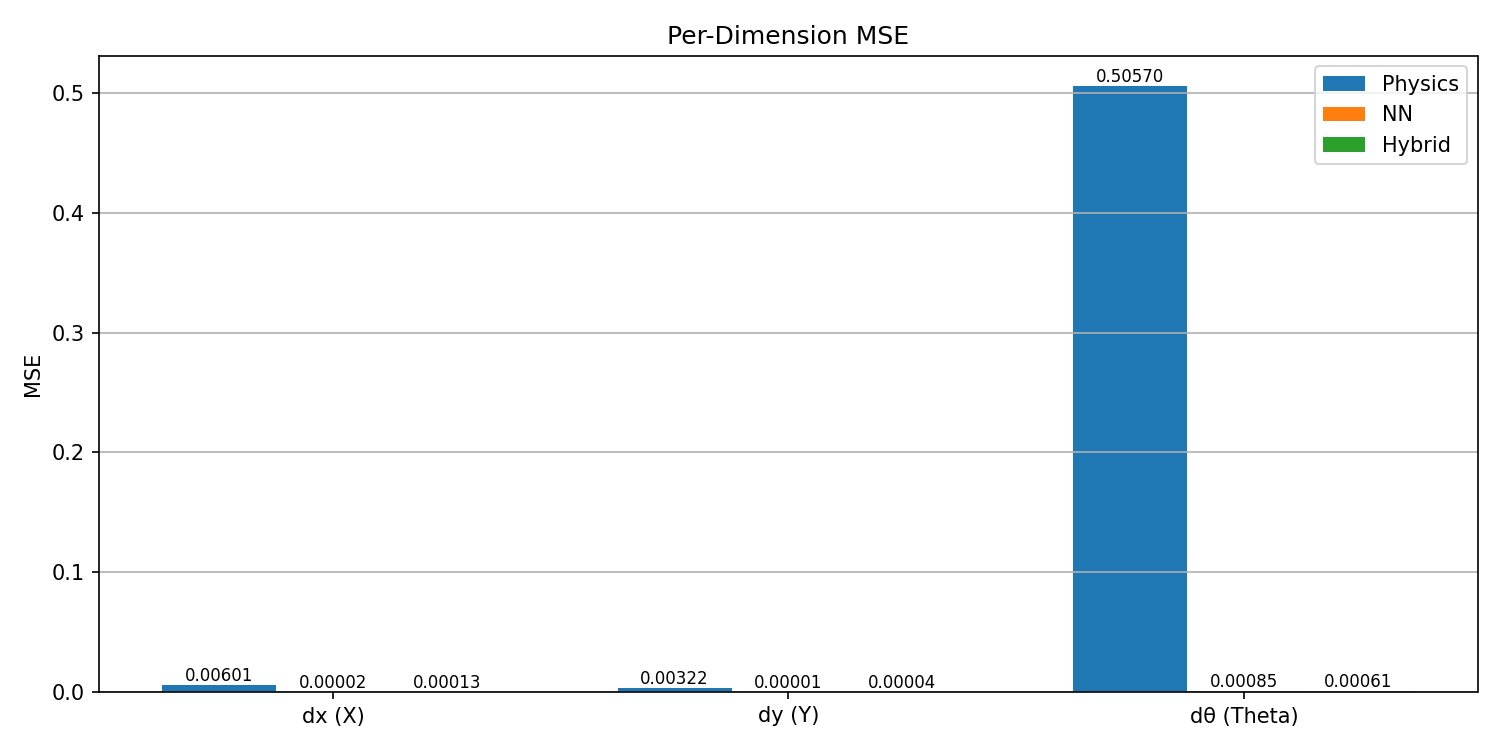
\includegraphics[width=\textwidth]{per_dim_mse.png}
    \caption{Per-dimension MSE breakdown. The physics model's error is dominated by the angular dimension ($d\theta$ MSE $= 0.5057$). Both the NN and Hybrid models reduce all dimensions by orders of magnitude, with the Hybrid achieving the best $d\theta$ performance.}
    \label{fig:per_dim}
\end{figure}

\begin{figure}[H]
    \centering
    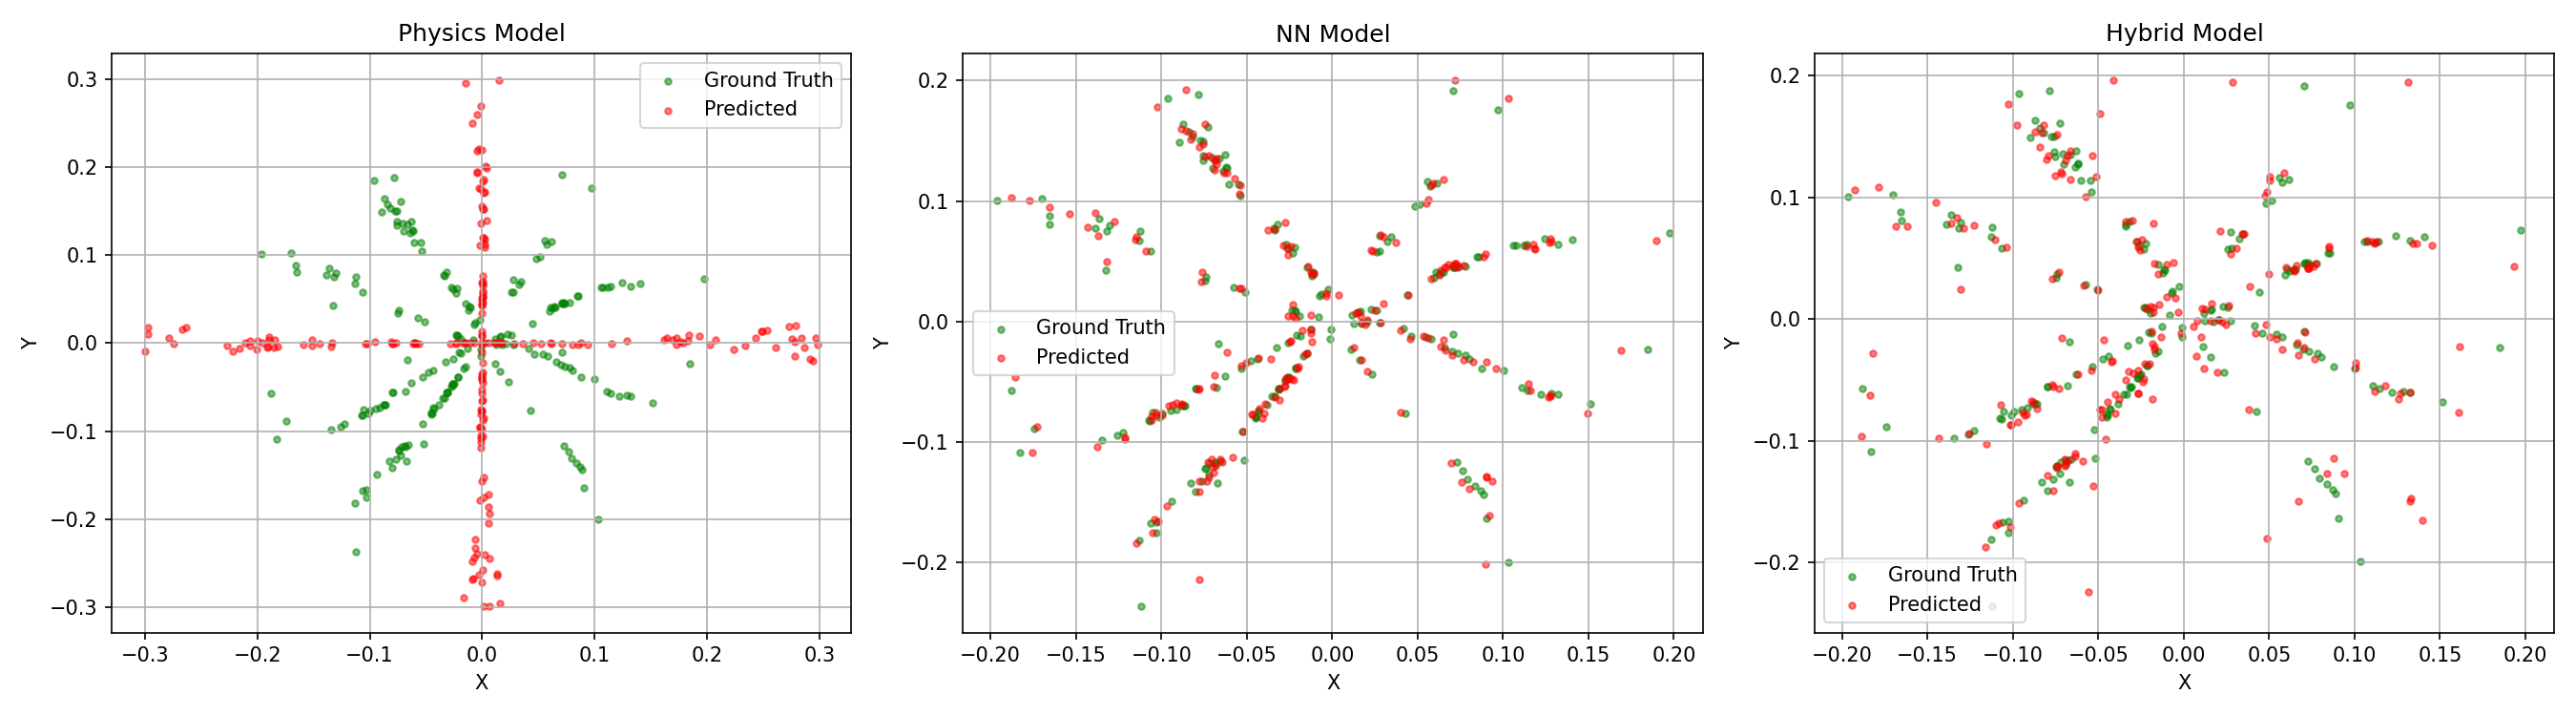
\includegraphics[width=\textwidth]{predictions.png}
    \caption{Scatter plots of predicted vs.\ ground-truth $(\Delta x, \Delta y)$ for all three models. The physics model (left) shows systematic bias; the NN (center) and Hybrid (right) show tight clustering around ground truth.}
    \label{fig:predictions}
\end{figure}

\subsection{Analysis of Each Approach}

\textbf{Physics Model.} \textit{Strengths:} Fully interpretable, requires no training data, and all parameters have clear physical meaning ($m$, $s$, $I$). It is dimensionally consistent and can generalize to different objects by changing the physical constants. \textit{Limitations:} The idealized rigid-body equations assume point contact, a square inertia profile ($I = \tfrac{1}{12}ms^2$), and no friction losses. The cracker box is rectangular, contact is distributed, and surface friction significantly affects the dynamics. Angular prediction is particularly poor (MSE $= 0.5057$), with the model under-predicting rotation by nearly an order of magnitude.

\textbf{Neural Network.} \textit{Strengths:} Achieves $580\times$ lower error than physics by learning the true input-output mapping from data. The trigonometric feature engineering captures the periodic structure of the dynamics without requiring knowledge of the underlying physics. L-BFGS fine-tuning provides further refinement. \textit{Limitations:} Purely data-driven---performance may degrade outside the training distribution. The model is a black box with no physical interpretability.

\textbf{Hybrid Model.} \textit{Strengths:} Best overall performance by combining the structural prior of physics with the flexibility of neural networks. The residual formulation means the network only needs to learn the correction $\hat{\mathbf{y}} - \hat{\mathbf{y}}_{\text{phys}}$, which is easier than learning the full dynamics from scratch. Even though the physics model is quite inaccurate (MSE $= 0.1716$), it still provides useful signal about the direction and approximate scale of motion. \textit{Limitations:} Requires running the physics engine at inference time. The improvement over the pure NN is modest ($1.1\times$), suggesting that the well-engineered feature transform already captures most of the periodic structure that the physics provides.

\subsection{When to Prefer Each Model}

\begin{itemize}
    \item \textbf{Physics model}: Best when training data is scarce or unavailable, when operating outside the data distribution, or when interpretability is critical.
    \item \textbf{NN model}: Best when abundant training data is available and maximum accuracy within the training distribution is needed with minimal inference complexity.
    \item \textbf{Hybrid model}: Best when maximum accuracy is required and a reasonable physics model exists. Particularly advantageous when training data is limited, as the physics prior regularizes the learning problem.
\end{itemize}


%=============================================================================
\section{Implementation Details}
%=============================================================================

\subsection{Project Structure}

\begin{verbatim}
src/
  config/default.yaml       # Hyperparameters and physics constants
  lib/models.py             # NNModel, NNPhysicsModel, FeatureTransform
  lib/physics.py            # PushPhysics engine
  helpers/utils.py          # Data loading, DataLoader preparation
  helpers/config.py         # YAML config loading, device management
  main.py                   # Full training pipeline and visualization
  train.py                  # train_model() and finetune_lbfgs()
  results/                  # Output plots
\end{verbatim}

\subsection{Hyperparameters}

\begin{table}[H]
\centering
\ra{1.3}
\caption{Hyperparameter configuration.}
\label{tab:hyperparams}
\begin{tabular}{@{}ll@{}}
\toprule
\textbf{Parameter} & \textbf{Value} \\
\midrule
Hidden dimensions & [64, 64] \\
Learning rate (Adam) & 0.001 \\
Weight decay & $10^{-4}$ \\
Batch size & 64 \\
Max epochs & 3000 \\
Early stopping patience & 500 \\
Warmup epochs & 50 \\
L-BFGS learning rate & 0.1 \\
L-BFGS max iterations & 1000 \\
Gradient clipping norm & 1.0 \\
\midrule
Mass $m$ & 0.1 kg \\
Size $s$ & 0.1 m \\
Inertia $I = \tfrac{1}{12}ms^2$ & $8.33 \times 10^{-5}$ kg$\cdot$m$^2$ \\
Simulation steps & 300 \\
Push duration $T$ & 3.0 s \\
\bottomrule
\end{tabular}
\end{table}

\subsection{Software}

The implementation uses PyTorch 2.4.0 with CUDA 12.1 for GPU-accelerated training, NumPy for data handling, and Matplotlib for visualization. The training pipeline employs a warmup-cosine learning rate schedule for stable convergence and L-BFGS second-order fine-tuning with Strong Wolfe line search for improved final performance.


%=============================================================================
\section{Conclusion}
%=============================================================================

We implemented and compared three approaches for predicting push dynamics of a cracker box. The physics model, using dimensionally consistent rigid-body dynamics ($\tau = mvd$, $\alpha = \tau/I$, $\Delta\theta = \frac{1}{2}\alpha\Delta t^2$), provides an interpretable but limited baseline (MSE $= 0.1716$), with the primary weakness being angular prediction due to unmodeled friction and geometry effects. The neural network achieves a $580\times$ improvement (MSE $= 0.000296$) through trigonometric feature engineering and L-BFGS fine-tuning. The hybrid model achieves the best results (MSE $= 0.000262$, $655\times$ improvement) by learning residual corrections to the physics predictions, demonstrating that even an imperfect physics model provides useful structural priors for data-driven learning in robotic manipulation.


\end{document}
